\section{Introduction\label{arr_sec:intro}}
% ===================

Given a set $\calC$ of planar curves, the {\em arrangement}
$\calA(\calC)$ is the subdivision of the plane into zero-dimensional,
one-dimensional and two-dimensional cells, called {\em vertices}, {\em
edges} and {\em faces}, respectively induced by the curves in $\calC$.
Arrangements are ubiquitous in the computational-geometry
literature and have many applications;
see, e.g.,~\cite{as-aa-00,cgal:h-a-04}.

The curves in $\calC$ can intersect each other (a single curve may also
be self-intersecting or may be comprised of several disconnected branches)
and are not necessarily $x$-monotone.\footnote{A continuous planar curve $C$
is {\em $x$-monotone} if every vertical line intersects it at
most once. For example, a non-vertical line segment is always
$x$-monotone and so is the graph of any continuous function $y = f(x)$.
For convenience, we treat vertical line segments as {\em weakly
$x$-monotone}, as there exists a single vertical line that overlaps them.
A circle of radius $r$ centered at $(x_0, y_0)$ is not $x$-monotone, as
the vertical line $x = x_0$ intersects it at $(x_0, y_0 - r)$ and at
$(x_0, y_0 + r)$.}
We construct a collection $\calC''$ of
$x$-monotone subcurves that are pairwise disjoint in their interiors
in two steps as follows. First, we decompose each curve in $\calC$
into maximal $x$-monotone subcurves (and possibly isolated points),
obtaining the collection $\calC'$. Note that an $x$-monotone curve cannot
be self-intersecting. Then, we decompose each curve in $\calC'$ into
maximal connected subcurves not intersecting any other
curve (or point) in $\calC'$. The collection $\calC''$ may also
contain isolated points, if the curves of $\calC$ contain such
points. The arrangement induced by the collection $\calC''$ can be
conveniently embedded as a planar graph, whose vertices are associated
with curve endpoints or with isolated points, and whose edges are
associated with subcurves. It is easy to see that
$\calA(\calC) = \calA(\calC'')$. This graph can be represented using a
{\em doubly-connected edge list} data-structure (\dcel\ for short),
which consists of containers of vertices, edges and faces and
maintains the incidence relations among these objects.

The main idea behind the \dcel\ data-structure is to represent
each edge using a pair of directed {\em halfedges}, one going from
the $xy$-lexicographically smaller (left) endpoint of the curve toward
its the $xy$-lexicographically larger (right) endpoint, and the other,
known as its {\em twin} halfedge, going in the opposite direction. As each
halfedge is directed, we say it has a {\em source} vertex and a {\em target}
vertex. Halfedges are used to separate faces, and to
connect vertices (with the exception of {\em isolated vertices}, which
are unconnected).

If a vertex $v$ is the target of a halfedge $e$, we say that $v$
and $e$ are {\em incident} to each other. The halfedges incident
to a vertex $v$ form a circular list oriented in a clockwise order
around this vertex. (An isolated vertex has no incident halfedges.)

Each halfedge $e$ stores a pointer to its {\it incident face},
which is the face lying to its left. Moreover, every halfedge is
followed by another halfedge sharing the same incident face, such
that the target vertex of the halfedge is the same as the source
vertex of the next halfedge. The halfedges are therefore connected
in circular lists, and form chains, such that all edges of a chain
are incident to the same face and wind along its boundary. We call
such a chain a {\em connected component of the boundary} (or {\em
CCB} for short).

The unique CCB of halfedges winding in a counterclockwise orientation
along a face boundary is referred to as the {\em outer CCB} of the
face. For the time being let us consider only arrangements of
bounded curves, such that exactly one unbounded face exists in every
arrangement. The unbounded face does not have an outer boundary. Any
other connected component of the boundary of the face is called a
{\em hole} (or {\em inner CCB}), and can be represented as a circular
chain of halfedges winding in a clockwise orientation around it.
Note that a hole does not necessarily correspond to a single face,
as it may have no area, or alternatively it may consist of several
connected faces. Every face can have several holes contained in its
interior (or no holes at all). In addition, every face may contain
isolated vertices in its interior. See Figure~\ref{arr_fig:seg_dcel}
for an illustration of the various \dcel\ features. For more details
on the \dcel\ data structure see~\cite[Chapter~2]{bkos-cgaa-00}.

\begin{figure}[t]
\begin{ccTexOnly}
  \begin{center}
  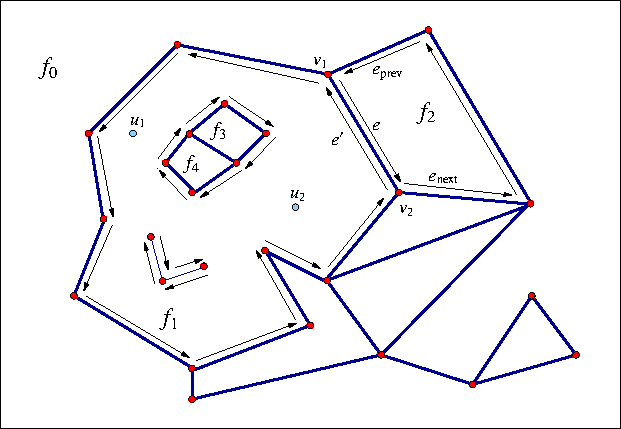
\includegraphics{Arrangement_on_surface_2/fig/arr_segs}
  \end{center}
\end{ccTexOnly}
\begin{ccHtmlOnly}
  <p><center>
  <img src="./fig/arr_segs.gif" border=0 alt="Arrangement of sgements">
  </center>
\end{ccHtmlOnly}
\caption{An arrangement of interior-disjoint line segments with some
of the \dcel\ records that represent it. The unbounded face $f_0$ has
a single connected component that forms a hole inside it, and this hole
is comprised if several faces. The half-edge $e$ is directed from its
source vertex $v_1$ to its target vertex $v_2$. This edge, together with
its twin $e'$, correspond to a line segment that connects the points
associated with $v_1$ and $v_2$ and separates the face $f_1$ from $f_2$.
The predecessor $e_{\rm prev}$ and successor
$e_{\rm next}$ of $e$ are part of the chain that form the outer
boundary of the face $f_2$. The face $f_1$ has a more complicated
structure as it contains two holes in its interior: One hole
consists of two adjacent faces $f_3$ and $f_4$, while the other
hole is comprised of two edges. $f_1$ also contains two isolated
vertices $u_1$ and $u_2$ in its interior.\label{arr_fig:seg_dcel}}
\end{figure}

The rest of this chapter is organized as follows: In
Section~\ref{arr_sec:arr_class} we review in detail the interface
of the \ccc{Arrangement_2} class-template, which is the central
component in the arrangement package. In
Section~\ref{arr_sec:queries} we show how queries on an arrangement
can be issued. In Section~\ref{arr_sec:gl_funcs} we
review some important free (global) functions that operate on
arrangements, the most important ones being the free 
insertion-functions. Section~\ref{arr_sec:traits} contains detailed
descriptions of the various geometric traits classes included in
the arrangement package. Using these traits classes it is possible
to construct arrangements of different families of curves. In
Section~\ref{arr_sec:notif} we review the notification mechanism
that allows external classes to keep track of the changes that an
arrangement instance goes through. Section~\ref{arr_sec:ex_dcel}
explains how to extend the \dcel\ records, to store extra data
with them, and to efficiently update this data.
In Section~\ref{arr_sec:overlay} we introduce the fundamental
operation of overlaying two arrangements.
Section~\ref{arr_sec:arr_with_hist} describes the
\ccc{Arrangement_with_history_2} class-template that extends the
arrangement by storing additional history records with its curves.
Finally, in Section~\ref{arr_sec:io} we review the arrangement
input/output functions.
